% 2007 年重庆卷文科第 19 题：直三棱柱 ABC-A1B1C1，∠ABC=90°，AB=1，BC=3/2，AA1=2；
%   D 在 BB1 上且 BD=BB1/3，B1E⊥A1D 于 E。图中 E 位于 A1D 上、B1 的左下方。
% 来源 PDF：gaokaomath-src/普通高考/2007/2007重庆文.pdf
% SHA-256：a647b60227db10d70c5c3fbe72b6ffe2c8a0667b233695e55bb4f5a7cef633a6
% 原页：2007重庆文.pdf 第 1 页（A3 三栏）第 3 栏，书页码 357。
% 重绘依据：按原页 A1、C1、B1、E、D、A、B、C 的相对位置与虚实线重绘；
%   斜投影的深度偏移取 0.55，使 D（BB1 的三分之一处）与底面对角线 AC 在图上分开。
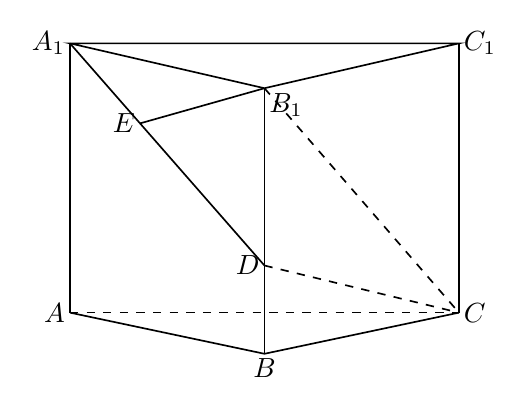
\begin{tikzpicture}[scale=0.95, semithick,
  every node/.style={inner sep=1.5pt}]

  \coordinate (A)  at (0.0,0.55);
  \coordinate (B)  at (2.60,0.00);
  \coordinate (C)  at (5.20,0.55);
  \coordinate (A1) at (0.0,4.15);
  \coordinate (B1) at (2.60,3.55);
  \coordinate (C1) at (5.20,4.15);
  \coordinate (D)  at (2.60,1.18);
  \coordinate (E)  at (0.936,3.08);

  % 底面
  \draw (A) -- (B) -- (C);
  \draw[dashed] (A) -- (C);
  % 侧棱
  \draw (A) -- (A1);
  \draw (B) -- (B1);
  \draw (C) -- (C1);
  % 上底面
  \draw (A1) -- (B1) -- (C1) -- cycle;

  % 题设连线
  \draw (A1) -- (D);
  \draw (B1) -- (E);
  \draw[dashed] (B1) -- (C);
  \draw[dashed] (D) -- (C);

  \node[left] at (A) {$A$};
  \node[below] at (B) {$B$};
  \node[right] at (C) {$C$};
  \node[left] at (A1) {$A_1$};
  \node[below right] at (B1) {$B_1$};
  \node[right] at (C1) {$C_1$};
  \node[left] at (D) {$D$};
  \node[left] at (E) {$E$};
\end{tikzpicture}
